\documentclass{article}

\usepackage{../../austin137}
\usepackage{../../local}
\usehyperstuff

\usepackage{wrapfig}

\begin{document}

%%%%%%%%%%%%%%%%%%%%%%%%%%%%%%%%%%%%%%%%%%%%%%%%%%%%%%%%%%%%%%%%%%%%%%%%%%%%%%%%
\addcopyright
\begin{center}
{\bf \large Physics W89 - Introduction to Mathematical Physics - Summer 2023}\\\medskip
{\bf \large Problem Set - Module 09 - One, Two, Three, Fourier} \\\medskip
{\emph{Last Update: \today}}
\end{center}

\dphline\bigskip
%%%%%%%%%%%%%%%%%%%%%%%%%%%%%%%%%%%%%%%%%%%%%%%%%%%%%%%%%%%%%%%%%%%%%%%%%%%%%%%%
\section*{Problem 9.1 - The Legendre Polynomials}
\relevid{Power Series Solutions; The Method of Frobeneus}

\paragraph{}
The \heavydef{Legendre polynomials} $P_{\ell}(x)$ are solutions to the second-order ODE
	\begin{equation}
		(1-x^{2})y'' - 2xy' + \ell(\ell+1)y = 0.
	\label{ODEtoP}
	\end{equation}

\paragraph{(a)}
Use the ansatz $y(x) = ax^{2}+bx+c$ to try to find solutions for this ODE in the three different cases $\ell = 0$, $\ell=1$, and $\ell=2$.\\
\note{You will only get a single solution using this ansatz for each of these cases since the other linearly independent solution is not a polynomial of finite order.}

\begin{solution}
	Using the Antsatz, we find $y''(x) = 2a$ and $y'(x) = 2ax + b$. Starting with $\ell = 0$, let's plug this
	in:
	\begin{align*}
		(1-x^2)(2a) - 2x(2ax + b) &= 0 \\
		-3ax^2 - bx + a = 0
	\end{align*}	
	Comparing coefficients, we realize that all the coefficients on the left hand side must be zero, Hence, 
	we get that $a = b = 0$, but $c$ can be anything, so any equation of the form $y = c$ where $c$ is 
	a constant solves the equation.

	For $\ell = 1$: 
	\begin{align*}
		(1-x^2)(2a) - 2x(2ax + b) + 2(ax^2+ bx + c) &= 0 \\
		-2ax^2 + (a + c) &= 0
	\end{align*}
	So from here we get that $a=0$ and $a+c=0$, but since $a = 0$ this means that $c = 0$ too. Since this 
	doesn't restrict anything on $b$, so the equation $y = bx$ for any $b$ would work. 

	Finally for $\ell = 2$:
	\begin{align*}
		(1-x^2)(2a) - 2x(2ax + b) + 6(ax^2 + bx + c) &= 0 \\
		2bx + 3c + a = 0
	\end{align*}
	From here we get that $b =0$, and $a + 3c = 0$, so this implies that $a=-3c$. Thus, any equation of 
	the form $y = ax^2-\frac{1}{3}a$ would satisfy this differential equation.
\end{solution}

\phline
%%%%%%%%%%%%%%%%%%%%%
\paragraph{}
We can solve Eq.~\ref{ODEtoP} by a power series solution using the Frobenius method!  Recall that this involves the ansatz
	\begin{equation*}
		y(x) = x^{r}\sum_{m=0}a_{m}x^{m} = \sum_{m=0}a_{m}x^{r+m},
	\end{equation*}
where $r\in\mathbb{R}$ is some unknown initial power and $a_{0} \neq 0$.

\paragraph{(b)}
Plug the power series ansatz into Eq.~\ref{ODEtoP}.  Find the indical equation (the coefficient of
the $x^{r-2}$ terms) to determine the two possible values of $r$.
\spoileranspart{$r$ can be 0 or 1}.

\begin{solution}
	Taking derivatives:
	\begin{align*}
		y'(x) &= \sum_m (r+m) a_m x^{r + m - 1}\\
		y''(x) &= \sum_m (r+m)(r+m-1)a_m x^{r + m-2} 
	\end{align*}
	Therefore our differential equation is:
	\[
		(1-x^2) \sum_m (r+m)(r+m-1)a_m x^{r+m-2} - 2x\sum_m (r+m)a_m x^{r+m-1} + \ell(\ell+1)\sum_m a_m
		x^{r+m} = 0 
	\]
	Expanding out the $1-x^2$:
	\begin{multline*}
		-\sum_m (r+m)(r+m-1)a_mx^{r+m} + \sum_m (r+m)(r+m-1)a_mx^{r+m-2} \\- 2\sum_m (r+m) a_m x^{r+m} +
		\ell(\ell+1)\sum_m a_m x^{r+m} = 0
	\end{multline*}
	For the indical equation, we set $m=0$, giving us:
	\[
		a_0x^r r(r-1) + r(r-1)a_0x^{r-2}- 2ra_0 x^r + \ell(\ell+1)a_0x^r = 0
	\] 
	Looking at the coefficient on the $x^{r-2}$ term, we have the equation $r(r-1)a_0 = 0$, but since $a_0 
	\neq 0$, this requires that $r(r-1) = 0$, so hence $r$ can be either $0$ or $1$, as confirmed by the spoiler.
\end{solution}

\paragraph{(c)} 
Find the equation for the coefficient of the $x^{r-1}$ terms.  Show that in the case (spoilers!) $r=0$ from part (b) that the coefficient $a_{1}$ may be left arbitrary
but in the case $r=1$, we must have $a_{1} = 0$.

\begin{solution}
	Looking at the equation we got from plugging in our Ansatz: 
	\[
	-\sum_m (r+m)(r+m-1)a_mx^{r+m} + \sum_m (r+m)(r+m-1)a_mx^{r+m-2} - 2\sum_m (r+m) a_m x^{r+m} +
		\ell(\ell+1)\sum_m a_m x^{r+m} = 0
	\]
	Here, only the second term in this entire expression has an $x^{r-1}$ exponent, when $m = 1$. Therefore, 
	we get the equation:
	\[
		r(r+1)a_1 x^{r-1} = 0
	\] 
	Here, if $r =0$, then $a_1$ can be anything, since the product equals zero regardless. However, if $r=1$, 
	then we have $2a_1 = 0$, meaning that $a_1$ must equal zero. 
\end{solution}
\paragraph{(d)}
Set the coefficients of the $x^{r+m}$ terms ($m\geq 0$) to zero to get a \heavydef{recursion relation} relating $a_{m+2}$ to $a_{m}$.  Then, 
in the case $\ell = 4$, $r = 0$, and $a_{1} = 0$, find all the non-zero coefficients in terms of $a_{0}$.  
Write down the solution $P_{4}(x)$ and check that it solves Eq.~\ref{ODEtoP}.

\begin{solution}
	To get the $x^{r+m}$ term, we first shift the indexing of the second term by 2, so that all the exponents
	on the $x$ are in line with each other:
	\begin{multline*}
		-\sum_{m=0} (r+m)(r+m-1)a_mx^{r+m} + \sum_{m = -2}(r+m+2)(r+m+1)a_{m+2}x^{r+m} \\- 2\sum_{m = 0}(r+m)
		a_mx^{r+m} + \ell(\ell+1)\sum_{m = 0} a_m x^{r+m} = 0
	\end{multline*}
	Pulling $x^{r+m}$ out of the equation, we notice that all the coefficients must be zero, which leaves
	us with the following equation (I'm intentionally skipping the algebra here since its a lot to type):
	\[
		-(r+m)(r+m-1)a_m + (r+m+2)(r+m+1)a_{m+2} - 2(r+m)a_m + \ell(\ell+1) a_m = 0
	\] 
	Solving for $a_{m+2}$, this gives:
	\[
		a_{m+2} = \frac{2(r+m) + (r+m)(r+m+1) - \ell(\ell+1)}{(r+m+2)(r+m+1)}a_m 
	\] 
	Now for our specific case of $\ell=4$, $r = 0$ and $a_1 = 0$, the recursion relation becomes:
	\[
		a_{m+2} = \frac{2m+m(m-1) - 20}{(m+1)(m+2)}a_m
	\] 
	Since $a_1 = 0$, and all odd terms $a_3, a_5, \dots, a_{2n +1}$ all depend on $a_1$, we conclude that 
	all odd coefficients $a_{2n+1} = 0$. To find $a_2$, we plug in $m =0$:
	\[
	a_2 = -\frac{20}{2} = -10a_0
	\] 
	Then to find $a_4$, we plug in $m=2$:
	\[
		a_4 = \frac{4 +2 - 20}{12} = -\frac{14}{12} = -\frac{7}{6}a_2 = -\frac{7}{6}(-10a_0) = \frac{35}{3}a_0
	\] 
	When we look to find $a_6$, we get:
	\[
		a_6 = \frac{8 + 12 - 20}{30} a_4 = 0
	\] 
	And since all subsequent even terms depend on $a_6$ (recursively), then we conclude that all the remaining
	terms here must be zero. Therefore, we've found all the nonzero coefficients. So writing out $P_4(x)$:
	\[
	P_4(x) = \frac{35}{3}a_0x^4 -10a_0x^2 + a_0
	\] 
	Computing its derivatives:
	\begin{align*}
		P_4'(x) &= \frac{140}{3}a_0x^3 - 20a_0x\\
		P_4''(x) &= 140a_0x^2 - 20a_0 
	\end{align*}
	Plugging this into the differential equation:
	\begin{multline*}
		(1-x^2)(140a_0x^2 - 20a_0) - 2x\left( \frac{140}{3}a_0x^3 - 20a_0x \right) + 20\left( \frac{35}{3}a_0x^4 - 10a_0x^2 + a_0 \right) \\= 140a_0x^2 - 20a_0 - 140a_0x^4 + 20a_0x^2 - \frac{280}{3}a_0x^4 + 40a_0x^2 + \frac{700}{3}a_0x^4 - 200a_0x^2 + 20a_0
	\end{multline*}
	Grouping terms:
	\[
	a_0x^4\left( \frac{700}{3} - \frac{280}{3} - 140\right) + a_0x^2(140 + 20 + 40 - 200) - a_0(20 - 20) = 0x^4 + 0x^2 + 0 = 0 
	\] 
	And since this all equals zero, we conclude that this indeed solves the differential equation.
\end{solution}
\bigskip
\dphline
\pagebreak
%%%%%%%%%%%%%%%%%%%%%%%%%%%%%%%%%%%%%%%%%%%%%%%%%%%%%%%%%%%%%%%%%%%%%%%%%%%%%%%%
\section*{Problem 9.2 - Trigonometric Fourier Series}
\relevid{The Trigonometric Fourier Series}

\paragraph{}
Consider the space of periodic functions of period $2\pi$.   This is a vector subspace of the vector space of functions of the variable $\theta$,
	\begin{equation*}
		\left.\left\{\vec{f}\doteq f(\theta)\,\right|f(\theta+2\pi)=f(\theta)\right\}.
	\end{equation*}
We can introduce the following inner product on the subspace of periodic functions,\footnote{Since the functions are periodic the range of integration can be
any $2\pi$ interval such as $-\pi$ to $\pi$ or $0$ to $2\pi$.}
	\begin{equation*}
		\vec{f}\bcdot\vec{g} \equiv \frac{1}{\pi}\int_{-\pi}^{\pi} f(\theta)^{*}g(\theta)d\theta.
	\end{equation*}
In class we introduced the basis vectors $\{\vec{e}_{0},\hat{e}_{c,n},\hat{e}_{s,n}\}$, with $n\in\mathbb{N}$,
	\begin{equation*}
		\vec{e}_{0} \doteq \fracsm{1}{2};	\qquad 	\hat{e}_{c,n} \doteq \cos(n\theta);	\qquad 	\hat{e}_{s,n} \doteq \sin(n\theta).
	\end{equation*}

%%%%%%%%%%%%%%%%%%%%%
\paragraph{(a)}		\extrapart
Show that the space of periodic functions of period $2\pi$ is indeed a vector subspace of the vector space of functions.


%%%%%%%%%%%%%%%%%%%%%
\paragraph{(b)}		
Show that $\{\vec{e}_{0},\hat{e}_{c,n},\hat{e}_{s,n}\}$ is an orthogonal set of functions under the inner product given and that 
$\hat{e}_{c,n}$ and $\hat{e}_{s,n}$ are normalized.  What is the normalization of $\vec{e}_{0}$?

\begin{solution}
	To prove they are orthogonal, we show that the inner product between all three of these equals zero. First,
	we start with $\hat{e}_0 \cdot \hat{e}_{s, n}$: 
	\begin{align*}
		\vec{e}_0 \cdot \hat{e}_{s, n} &= \frac{1}{\pi}\int_{-\pi}^\pi \frac{1}{2}\sin(n \theta) d\theta  \\
									   &= \frac{1}{2\pi n}\left( -\cos(n \theta) \right)_{-\pi}^\pi \\
									   &= \frac{1}{2\pi n}\left[-\cos(n \pi) + \cos(-n\pi)\right] 
	\end{align*}
	Since the cosine function is even, we have $\cos(x) = \cos(-x)$, so the term in the square brackets cancels
	out, and we get $\hat{e}_0 \cdot \hat{e}_{s, n} = 0$. Now for $\hat{e}_0 \cdot \hat{e}_{c, n}$:
	\begin{align*}
		\vec{e}_0 \cdot \hat{e}_{c, n} &= \frac{1}{\pi}\int_{-\pi}^\pi \frac{1}{2}\cos(n \theta) d\theta \\
									   &= \frac{1}{2\pi n}(\sin (n \theta))_{-\pi}^\pi  \\
									   &= \frac{1}{2\pi n}(2 \sin(n \pi)) \\
									   &= \frac{\sin (n\pi)}{\pi n} 
	\end{align*}
	And since $n$ is an integer, $\sin(n\pi) = 0$, so therefore $\hat{e}_0 \cdot \hat{e}_{c, n} = 0$. Finally, 
	for $\hat{e}_{c, n} \cdot \hat{e}_{s, n}$:
	\begin{align*}
		\hat{e}_{c, n} \cdot \hat{e}_{s, n} &= \frac{1}{\pi} \int_{-\pi}^\pi \cos(n \theta) \sin(n \theta) d\theta
	\end{align*}
	Here we can so a u-substitution of $u = \sin(n \theta)$, so $du = n \cos(n \theta) d\theta$, therefore:
	\[
		\hat{e}_{c, n} \cdot \hat{e}_{s, n} = \int_{0}^{0} \frac{1}{n} du = 0
	\] 
	This integral is equal to zero since we're integrating over a region of zero width. Hence, we've proven that
	every basis vector is orthogonal to one another. To show that the $\hat{e}_{c,n}$ and $\hat{e}_{s, n}$ are
	normalized, we take the inner product with themselves, here I used Mathematica to compute these integrals
	since I couldn't figure these out by hand:
	\[
		\hat{e}_{c,n} \cdot \hat{e}_{c,n} = \frac{1}{\pi}\int_{-\pi}^\pi \cos^2(n \theta) d\theta = \frac{1}{\pi}\left( \pi + \frac{\sin(2n \pi)}{2n}\right) = \frac{1}{\pi} \pi = 1
	\] 
	Now for sine:
	\[
		\hat{e}_{s, n} \cdot \hat{e}_{s, n} = \frac{1}{\pi}\int_{-\pi}^\pi \sin^2(n \theta) d\theta = \frac{1}{\pi}\left( \pi - \frac{\sin(2 n \pi)}{2n} \right) = \frac{1}{\pi}\pi = 1
	\] 
	As for the normalization of $\hat{e}_0$, 
	all we have to do is find the inner product of $\hat{e}_0$ with itself:
	\[
		\vec{e}_0 \cdot \vec{e}_0 = \frac{1}{\pi}\int_{-\pi}^\pi \frac{1}{4}d \theta = \frac{1}{4\pi}(2\pi) = \frac{1}{2}
	\] 
	As for the ``length'' of the vector, we can take the square root of this quantity:
	\[
	|\vec{e}_0| = \frac{1}{\sqrt{2} } 
	\] 
	so if we want to find $\hat{e}_0$, we take $\vec e_0$ and divide it by the magnitude:
	\[
	\hat{e}_0 = \frac{\frac{1}{2}}{\frac{1}{\sqrt{2} }} = \frac{1}{\sqrt{2} }  
	\] 
	and that completes the problem.
\end{solution}

\phline
%%%%%%%%%%%%%%%%%%%%%
\paragraph{}
Any arbitrary real periodic function $f(\theta)$ of period $2\pi$ can be written with respect to this basis which results in the \heavydef{trigonometric Fourier expansion} of $f(\theta)$:
	\begin{align}
		\vec{f} &= a_{0}\vec{e}_{0} + \sum_{n=1}^{\infty}a_{n}\hat{e}_{c,n} + \sum_{n=1}^{\infty}b_{n}\hat{e}_{s,n}		\label{trigseries}\\	\eqimplies
		f(x) &=\fracsm{1}{2}a_{0} + \sum_{n=1}^{\infty} a_{n}\cos(n\theta) + \sum_{n=1}^{\infty} b_{n}\sin(n\theta).
	\label{trigexpansion}
	\end{align}

%%%%%%%%%%%%%%%%%%%%%
\paragraph{(c)}		\extrapart
Use the expression Eq.~\ref{trigseries} given for $\vec{f}$ and the results from part (b) to show that the Fourier coefficients can be determined via the following expressions:
	\begin{equation*}
		a_{0} = 2\vec{e}_{0}\bcdot\vec{f},	\qquad	a_{n} = \hat{e}_{c,n}\bcdot{\vec{f}},		\qquad b_{n} = \hat{e}_{s,n} \bcdot\vec{f}.
	\end{equation*}

\phline
%%%%%%%%%%%%%%%%%%%%%
\paragraph{}
Given the result of part (c) we can find the coefficients using the integral expression of the dot product.  For example, 
$a_{2} = \hat{e}_{c,2}\bcdot{\vec{f}} = \frac{1}{\pi}\int_{-\pi}^{\pi} \cos(2\theta)f(\theta)dx$.

%%%%%%%%%%%%%%%%%%%%%
\paragraph{(d)}
Use symmetry to determine which coefficients are zero for \heavydef{even functions}, $f(-\theta) = f(\theta)$.  For \heavydef{odd functions}, $f(-\theta) = -f(\theta)$?

\begin{solution}
	For $a_0$, we have:
	\[
		a_0 = \frac{2}{\pi}\int_{-\pi}^\pi \frac{1}{2}f(\theta) d\theta 
	\] 
	Since the integral is over a symmetric interval, we get that an odd $f(\theta)$
	will give us zero, while even functions will be nonzero. 

	For $a_n$, we have:
	\[
		a_n = \frac{1}{\pi}\int_{-\pi}^\pi \cos(n \theta) f(\theta) d\theta 
	\] 
	Since $\cos(n \theta)$ is even, and the product of an even function and an odd function is odd, then we 
	find that odd functions will have all $a_n = 0$, while even functions will be nonzero. 

	Finally, for $b_n$:
	\[
		b_n = \frac{1}{\pi}\int_{-\pi}^\pi \sin(n \theta) f(\theta) d\theta 
	\] 
	We find the exact opposite is the case. Since $\sin(n\theta)$ is an odd function, we find that if $f(\theta)$
	is even then $b_n = 0$, while odd functions have nonzero $b_n$. 
\end{solution}

%%%%%%%%%%%%%%%%%%%%%
\paragraph{(e)}
What are the trigonometric Fourier coefficients $\{a_{0},a_{n},b_{n}\}$ for the function $f(\theta) = \cos(3\theta)$?  $f(\theta) = \sin(4\theta)$?  $f(\theta) = e^{2i\theta}$?
\spoilers{You can basically just read these off!  For the last one, use Euler's formula.}

\begin{solution}
	Following the spoiler, we can just read these off. Since the expansion is:
	\[
	f(x) = \frac{1}{2}a_0 + \sum_n a_n \cos(n \theta) + \sum_n b_n \sin(n \theta)
	\] 
	the function $f(\theta) = \cos(3 \theta)$ has $a_3 = 1$, and all other $a_n, b_n = 0$. Likewise, for 
	$f(\theta) = \sin(4 \theta)$ we have $b_4 = 1$, with all other $a_n, b_n = 0$. Finally, with $f(\theta) = 
	e^{2 i \theta}$, we use Euler's formula to rewrite this as:
	\[
		e^{2 i \theta} = \cos(2\theta) + i \sin(2 \theta)
	\] 
	So this means that $a_2 = 1$, $b_2 = i$, and all other $a_n, b_n = 0$.
\end{solution}

%%%%%%%%%%%%%%%%%%%%%
\paragraph{(f)}
Find the trigonometric Fourier coefficients for the \heavydef{square wave}, a periodic function defined so $f(\theta) = +1$ if $n\pi < \theta < (n+1)\pi$ and $n$ is an even integer and
$f(\theta) = -1$ if $n\pi < \theta < (n+1)\pi$ and $n$ is an odd integer.

\begin{solution}
	Here, we'll integrate the function from $0$ to $2\pi$ instead of $-\pi$ to $\pi$. The function 
	is odd over this interval, so from part (d), we know that $a_0 = 0$ and $a_n = 0$, since for them 
	to be nonzero we require an even function $f(\theta)$. All that remains is to calculate $b_n$:
	\begin{align*}
		b_n &= \hat{e}_{s, n} \cdot \vec f\\
			&= \frac{1}{\pi}\left[ \int_0^\pi \sin(n \theta) (1) d\theta + \int_\pi^{2\pi} \sin(n \theta) (-1) d\theta\right]
	\end{align*} 
	After some algebra, we get:
	\[
		b_n = \frac{2}{n\pi}\left[ 1 - (-1)^n\right]
	\] 
	This means that if $n$ is even, then $b_n = 0$, the term in the square brackets evaluates to zero. However, 
	if $b_n$ is odd, then
	\[
	b_n = \frac{4}{n\pi}
	\] 
	To write this more concisely:
		\[
	b_n = \begin{cases}
		\frac{4}{n\pi} & \text{$n$ odd}\\
		0 & \text{$n$ even}
	\end{cases}
	\]
	And that completes the problem.
\end{solution}

%%%%%%%%%%%%%%%%%%%%%
\paragraph{(g)}		\extrapart
Graph the square wave function and the approximations taken by only keeping the terms up to $n=1$, $n=3$, and $n=10$.


%%%%%%%%%%%%%%%%%%%%%
\paragraph{(h)}		\extrapart
What does taking the derivative of a function do to the trigonometric Fourier coefficients?  That is, if $f(x)$ has coefficients $\{a_{0},a_{n},b_{n}\}$, what are the coefficients
$\{\tilde{a}_{0},\tilde{a}_{n},\tilde{b}_{n}\}$ of $f'(\theta) = \frac{df}{d\theta}$?
\spoilers{Start with the expansion in Eq.~\ref{trigexpansion} and take the derivative.  Then you can just read off the coefficients of the cosines and signs.}

\bigskip
\dphline
\pagebreak
%%%%%%%%%%%%%%%%%%%%%%%%%%%%%%%%%%%%%%%%%%%%%%%%%%%%%%%%%%%%%%%%%%%%%%%%%%%%%%%%
\section*{Problem 9.3 - The Exponential Fourier Series}
\relevid{The Complex Fourier Series}

\paragraph{}
Consider the space of periodic functions of period $L = 2\pi/k_{0}$ or, equivalently, the space of functions defined on the interval 
$x_{0} \leq x \leq x_{0}+L$ so that the range of interest has width $L$.   
This is again a vector subspace of the vector space of functions. 
We can again make an inner product on this space,\footnote{It turns out that if $f(x)$ and $g(x)$ are periodic with period $L$ then this choice of starting point is irrelevant and doesn't
appear in any answers.}
	\begin{equation*}
		\vec{f}\bcdot\vec{g} = \frac{1}{L}\int_{x_{0}}^{x_{0}+L} f^{*}(x)g(x)dx.
	\end{equation*}
With respect to this inner product we have an orthonormal set of vectors $\{\hat{e}_{n}\}$, $n\in\mathbb{Z}$ for this subspace,
	\begin{equation*}
		\hat{e}_{n} \doteq e^{ink_{0}x},
	\end{equation*}
The \heavydef{exponential Fourier series} for a function is then the expansion of that function with respect to this basis,
	\begin{equation}
		\vec{f} = \sum_{n=-\infty}^{\infty} c_{n}\hat{e}_{n} 	\eqimplies		f(x) = \sum_{n=-\infty}^{\infty}c_{n}e^{ink_{0}x}.
	\label{expansion}
	\end{equation}
We can find the expansion coefficients using orthonormality of these basis vectors,
	\begin{equation}
		c_{n} = \hat{e}_{n}\bcdot\vec{f} = \frac{1}{L}\int_{x_{0}}^{x_{0}+L}e^{-ink_{0}x}f(x)\,dx.
	\label{components}	
	\end{equation}

%%%%%%%%%%%%%%%%%%%%%
\paragraph{(a)}	
Plug Eq.~\ref{expansion} into the right-side of Eq.~\ref{components} and use orthonormality
to show that the right-hand side of Eq.~\ref{components} does indeed evaluate to $c_{n}$.
\spoilers{You may assume orthonormality.  
Be careful!  You will have to change the summation index in Eq.~\ref{expansion} since we are already using the index $n$ in Eq.~\ref{components}.}

\begin{solution}
	Substituting the relevant equations in:
	\begin{align*}
		c_n &= \frac{1}{L}\int_{x_0}^{x_0+L} e^{-in k_0x} \sum_{n'} c_{n'} e^{i n' k_0x} dx\\
			&= \sum_{n'} c_{n'} \underbrace{\frac{1}{L}\int_{x_0}^{x_0+L} e^{-in k_0x} e^{in' k_0x} dx}_{=\hat{e}_n \cdot \hat{e}_{n'}}
	\end{align*}
	Now, notice that since our basis functions are exponentials $\hat{e}_n = e^{i nk_0x}$, then this integral
	is actually just the inner product of two basis vectors, or $\hat{e}_n \cdot \hat{e}_{n'}$. Hence, this 
	is equal to the delta function, so we have:
	\[
		\sum_{n'} c_n \delta_{nn'} = c_n
	\] 
	So the expression indeed gives us $c_n$. 
\end{solution}

%%%%%%%%%%%%%%%%%%%%%
\paragraph{(b)}		\extrapart
Show that if $f(x)$ is a real function then $c_{-n} = c_{n}^{*}$, and if $f(x) = \pm f(-x)$ then $c_{-n} = \pm c_{n}$.

\phline
%%%%%%%%%%%%%%%%%%%%%
\paragraph{}
	%~~~~~~~~~~~~~~ FIGURE ~~~~~~~~~~~~~~%
	\setlength{\intextsep}{10pt}%
	\begin{wrapfigure}[6]{r}{0cm}
		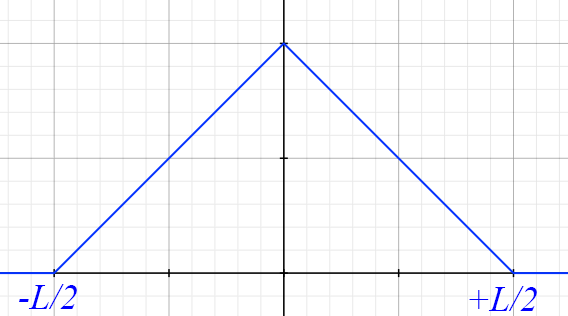
\includegraphics[width = 0.3\textwidth]{89-PS9-P3-Triangle}
	\end{wrapfigure}
	%~~~~~~~~~~~~~~ FIGURE ~~~~~~~~~~~~~~%
Consider a guitar string of length $L$ stretched from $-L/2$ to $+L/2$.  Let $x$ be the length along the string and let $y(x)$ be the height of the string.  Initially, the guitar string is ``plucked'' to a triangular shape,
	\begin{equation*}
		y(x) = \begin{cases} +x+\fracsm{L}{2},	& -\fracsm{L}{2}\leq x \leq 0\\[0.2cm]
		-x+\fracsm{L}{2},	& 0\leq x \leq \fracsm{L}{2} \end{cases}.
	\end{equation*}

\paragraph{(c)}
Find the Fourier expansion coefficients $c_{n}$ for this function.\\
\note{Our period here is $L$ and our interval starts at $x_{0} = -L/2$.}
\spoilers{Hmm... this seems awfully familiar..,}

\begin{solution}
	Here we just use the definition that $c_n = \hat{e}_n \cdot \vec f$:
	\begin{align*}
		c_n &= \frac{1}{L}\int_{-L / 2}^{L / 2} e^{-in k_0x} y(x) dx\\
			&= \frac{1}{L}\int_{-L / 2}^0 e^{-in k_0x}\left( x + \frac{L}{2} \right) dx + \frac{1}{L}\int_0^{L / 2} e^{-ink_0x}\left( -x + \frac{L}{2} \right) dx 
	\end{align*}
	Now we can use Mathematica to help us out with this integration:
	\[
		c_n = \frac{L(1 - e^{-in \pi} - in\pi)}{4n^2\pi^2} + \frac{L(1-e^{in \pi } + in \pi)}{4n^2\pi^2}
	\] 
	Adding these two up and simplifying, this gets us:
	\[
	c_n = \frac{L(1-\cos(\pi n))}{2n^2\pi^2}
	\] 
	Then, after plugging in that $L = \frac{2\pi}{k}$, we get:
	\[
	c_n = \frac{1 - \cos(\pi n)}{n^2 \pi k_0}
	\] 
\end{solution}
\phline
%%%%%%%%%%%%%%%%%%%%%
\paragraph{(d)}
What does taking the derivative of a function do to the exponential Fourier coefficients?  That is, if $f(x)$ has coefficients $\{c_{n}\}$, what are the coefficients
$\{\tilde{c}_{n}\}$ of $f'(x) = \frac{df}{dx}$?
\spoilers{Start with the expansion in Eq.~\ref{expansion} and take the derivative.  Then you can just read off the coefficients of the exponentials.}

\begin{solution}
	We can just take the derivative starting with the expression
	\[
		f(x) = \sum_{n =-\infty}^{\infty} c_n e^{in k_0x}
	\] 
	Simply taking the derivative (making use of its linearity):
	\[
		f'(x) = \sum_{n = -\infty}^\infty c_n (ink_0) e^{ink_0x}
	\] 
	So we get that $c_{n}' = c_n (ink_0)$.
\end{solution}

\bigskip
\dphline
\pagebreak
%%%%%%%%%%%%%%%%%%%%%%%%%%%%%%%%%%%%%%%%%%%%%%%%%%%%%%%%%%%%%%%%%%%%%%%%%%%%%%%%
\section*{Problem 9.4 - The Dirac Delta}
\relevid{The Fourier Transform; The Fourier Transform Completeness Relations (for a discussion of the Dirac Delta Function)}

\paragraph{}
Recall the following two integral relationships involving the Dirac delta function
	\begin{align}
		\int_{a}^{b} f(u)\delta(u-u_{0}) du &= \begin{cases} f(u_{0}), & a<u_{0}<b\\0,&\mbox{else}\end{cases};	\nonumber\\
		\qquad\quad \iinf e^{iau} du &= 2\pi\delta(a). \label{IntegralDelta}
	\end{align}
Also recall that the Fourier transform of a function of space (or time) $f(x)$ is given by a function of wavenumber (or frequency) $c(k)$ (also written $\mathcal{F}[f](k)$ or $F(k)$
or $\widetilde{f}(k)$), where
	\begin{align*}
		\textrm{Inverse Fourier Transform:}\qquad f(x) &=\frac{1}{2\pi}\iinf c(k)e^{ikx}dk,					\\		
		\textrm{Fourier Transform:}\qquad c(k) &= \iinf e^{-ikx}f(x)dx.		
	\end{align*}
{\bf{Warning:}} \emph{There are many different conventions for the definition of the Fourier transform, including how the $1/2\pi$ prefactor of the integrals is
split up and whether the cyclic or angular frequencies/wavenumbers are used.  This makes comparing between sources a pain.\footnote{Our convention puts the factor of
$1/2\pi$ on the Inverse Fourier transform formula, matching what Wikipedia calls the ``non-unitary convention'' with angular frequency.  Boaz notably uses a different
convention, with $1/2\pi$ on the Fourier transform formula instead.}  
See the Problem Set Supplement for a discussion of this.}

%%%%%%%%%%%%%%%%%%%%%
\paragraph{(a)}
Find the Fourier transforms of $\delta(x-x_{0})$, $e^{ik_{0}x}$, and $\sin(k_{0}x)$.  
Be sure to show all your work.\\
\note{Please try to do this one without looking at our lecture notes, which partially contain the solutions.}

\begin{solution}
	I'll do this in a list: 
	\begin{itemize}
		\item $f(x) = \delta(x - x_0)$: 
			\[
				c(k) = \int_{-\infty}^\infty e^{-ikx} \delta(x - x_0) = e^{-ikx_0}
			\] 
		\item $f(x) = e^{ik_0x}$: 
			\[
				c(k) = -\int_{-\infty}^\infty e^{-ikx} e^{ik_0x} = \int_{-\infty}^\infty e^{i(k_0-k)x} = 2\pi
				\delta(k_0-k) = 2\pi\delta(k - k_0)
			\] 
		\item $f(x) = \sin(k_0x)$
			\begin{align*}
				c(k) &= \int_{-\infty}^\infty e^{-ikx} \sin(k_0x) dx  \\
					 &= \frac{1}{2i}\int_{-\infty}^\infty e^{ikx}\left( e^{ik_0x} - e^{-ik_0x} \right)  \\
					 &= \frac{1}{2i} \left[ 2\pi\delta (k_0-k) - 2\pi\delta(k + k_0)\right]\\
					 &= \frac{\pi}{i}\left[\delta(k-k_0) - \delta(k+k_0)\right] 
			\end{align*}
	\end{itemize}
\end{solution}

%%%%%%%%%%%%%%%%%%%%%
\paragraph{(b)}		\extrapart
Use integration to prove the identity $\delta\big(a(x-x_{0})\big) = \frac{1}{\abs{a}}\delta(x-x_{0})$.\\  
\note{We did this in lecture.  Recall that a $u$-substitution is key to this proof.}


\phline
%%%%%%%%%%%%%%%%%%%%%
\paragraph{}
If there is more than one place where the argument of the delta function is zero, we have to be careful.  For example, we have the following identity, 
	\begin{equation*}
		\delta\big((x-x_{1})(x-x_{2})\big) = \frac{\delta(x-x_{1})+\delta(x-x_{2})}{\abs{x_{1}-x_{2}}}.
	\end{equation*}
Let's prove this identity by integrating!  Let $x_{1} < x_{2}$ and consider some constant $c$ between $x_{1}$ and $x_{2}$ so $x_{1}<c<x_{2}$.  Note that these are
all strict inequalities.

\paragraph{(c)}
Evaluate the integral $\iinf f(x)\delta\big((x-x_{1})(x-x_{2})\big)dx$ by breaking up the range of the integral to $-\infty$ to $c$ followed by $c$ to $+\infty$.  
Show that this gives the same answer as the integral $\iinf f(x)\frac{1}{\abs{x_{1}-x_{2}}}\big(\delta(x-x_{1})+\delta(x-x_{2})\big)dx$. 
\spoiler{The result from part (b) is key to this proof!  Note that in the region around $x=x_{1}$, we can effectively treat the term $(x-x_{2})$ as the constant $(x_{1}-x_{2})$.}

\begin{solution}
	Splitting the integral we get: 
	\[
		\int_{-\infty}^\infty f(x) \delta((x - x_1)(x - x_2)) dx = \int_{-\infty}^c f(x)
		\delta((x - x_1)(x - x_2)) dx + \int_c^\infty f(x) \delta((x - x_2) (x - x_1)) dx 
	\]
	Since $x_2$ is outside the bound of the first integral, the term $x - x_2$ can be treated as a constant, 
	and in the second integral, $x_1$ is outside the bound so $x - x_1$ is treated as a constant value. 
	Therefore, we can use the relation:
	\[
	\delta(a(x - x_0)) = \frac{1}{|a|}\delta(x - x_0)
	\] 
	 to simplify the expression. Doing so, we get: 
	 \begin{align*}
 \int_{-\infty}^c \frac{f(x)}{|x - x_2|}
 \delta(x - x_1) dx + \int_c^\infty \frac{f(x)}{|x - x_1|} \delta(x - x_2) dx &= \frac{f(x_1)}{|x_1 - x_2|} + \frac{f(x_2)}{|x_2 - x_1|}\\
 &= \frac{f(x_1) + f(x_2)}{|x_1 - x_2|} 
	 \end{align*}
	 Now the right hand side:
	 \begin{align*}
		 \int_{-\infty}^\infty f(x) \frac{1}{|x_1 - x_2|}(\delta(x - x_1) + \delta(x - x_2)) dx &= \frac{1}{|x_1 - x_2|}\left[\int_{-\infty}^\infty f(x) \delta( x - x_1) dx + \int_{-\infty}^\infty f(x) \delta(x - x_2) dx\right] \\
		 &= \frac{f(x_1) + f(x_2)}{|x_1 - x_2|} 
	 \end{align*}
	 which exactly matches the left hand side. Hence, we conclude that they are equal.
\end{solution}

\phline
%%%%%%%%%%%%%%%%%%%%%
\paragraph{}
The \heavydef{Heaviside step function}
(really another example of a distribution rather than a proper function) $\theta(x)$ may be defined as\footnote{There are different conventions for the value of $\theta(0)$.  
In our definition it's 1, in others it's 1/2.}
	\begin{equation*}
		\theta(x) \equiv \begin{cases} 1, & x\geq 0,\\ 0, & x<0\end{cases}.
	\end{equation*}
That is, the function is ``heavy'' on one side (1, when $x>0$) and ``light'' on the other (0, when $x<0$).\footnote{This is an example of an \heavydef{aptronym} - a name that is amusingly appropriate
to the application.  The Heaviside step function is actually named after mathematician and physicist Oliver Heaviside.} 
The Heaviside step function gives us a really convenient way to write some piecewise functions.  For example, the \heavydef{rectangle function} $\Pi(x)$ and 
\heavydef{ramp} function $R(x)$ can be expressed as
	\begin{align*}
		\Pi(x) &= \theta\left(x+\fracsm{1}{2}\right) - \theta\left(x-\fracsm{1}{2}\right) = \begin{cases} 1, & -\fracsm{1}{2} \leq x < \fracsm{1}{2},\\
		0, & \textrm{else}\end{cases}\\
		R(x) &= x\theta(x) = \begin{cases} x, & x\geq 0\\ 0, & x<0\end{cases}.
	\end{align*}

%%%%%%%%%%%%%%%%%%%%%
\paragraph{(d)}
Argue that the Heaviside step function can be used to ``encode'' the limits of integration into the integrand,
	\begin{equation*}
		\iinf f(x)\theta(x-a)dx = \int_{a}^{\infty}f(x)dx,	\qquad
		\iinf f(x)\theta(b-x)dx = \int_{-\infty}^{b}f(x)dx.
	\end{equation*}

	\begin{solution}
		For the first equation, notice that due to the definition of the Heaviside function, that 
		the integrand is only nonzero when $x > a$, so anything with $x < a$ will immediately equal zero, 
		and hence can be taken out of the integral. Therefore:
		\[
			\int_{-\infty}^\infty f(x) \theta(x - a) dx = \int_a^\infty f(x) dx 
		\] 
		For the second equation, it's the same deal except backwards. The integrand is only nonzero when 
		$b - x > 0$, or $x < b$, so this serves as an upper bound instead:
		\[
			\int_{-\infty}^\infty f(x) \theta(b - x) dx = \int_{-\infty}^b f(x) dx 
		\] 
	\end{solution}
\phline
%%%%%%%%%%%%%%%%%%%%%
\paragraph{(e)}
Show or argue that the integral of the Dirac delta is the Heaviside step function, $\theta(x) = \int_{-\infty}^{x} \delta(x')dx'$ and, conversely, that
the Dirac delta is the derivative of the Heaviside step function, $d\theta(x)/dx = \delta(x)$.
\extrasubpart{Show that the integral of the Heaviside step function is the Ramp function $R(x) = \int_{-\infty}^{x} \theta(x')dx'$ and, conversely, 
that the Heaviside step function is the derivative of the Ramp function,  $dR(x)/dx = \theta(x)$.}

\begin{solution}
	We start with the definition of the Dirac delta:
	\[
		\int_a^b f(u) \delta(u - u_0) du = \begin{cases} f(u_0) & a < u_0 < b\\
		0 & \text{else}\end{cases}
	\] 
	Now, we'll let $f(u) = 1$, let $b = x$, $a = -\infty$ and $u_0 = 0$ so that this equation 
	assumes the form given in the problem statement. Then, we get the equation:
	\[
		\int_{-\infty}^x \delta(u) du = \begin{cases}
			1 & -\infty < 0 < x\\
			0 & \text{else}
		\end{cases}
	\] 
	where the right hand side can be rewritten as:
	\[
		\int_{-\infty}^x \delta(u) du = \begin{cases}
			1 &		x > 0\\
			0 & \text{else}
		\end{cases} = \theta(x)
	\] 
	which is exactly the definition of the Heaviside step function. On the other side, we can see that the 
	Heaviside function is constant when $x < 0$ and $x > 0$ and hence has zero slope in these regions, 
	whereas at $x=0$ the function immediately jumps up to 1, which roughly translates to a slope of infinity. 
	This matches exactly the Dirac delta definition, where it's zero everywhere except at $x=0$, where
	its value can be interpreted as infinite.
\end{solution}


\bigskip
\dphline
\pagebreak
%%%%%%%%%%%%%%%%%%%%%%%%%%%%%%%%%%%%%%%%%%%%%%%%%%%%%%%%%%%%%%%%%%%%%%%%%%%%%%%%
\section*{Problem 9.5 - The Fourier Transform}
\relevid{The Fourier Transform;
Convolution}

\paragraph{}
For this problem, let's look at time-domain functions and their Fourier-transforms into frequency-domain functions,
	\begin{align}
		\mathcal{F}^{-1}[c(\omega)](t) = f(t) &= \frac{1}{2\pi}\iinf c(\omega)e^{i\omega t}d\omega,					\label{fouriert}\\
		\qquad\quad		
		\mathcal{F}[f(t)](\omega) = c(\omega) &= \iinf e^{-i\omega t} f(t)dt.		\label{inversefouriert}
	\end{align}

%%%%%%%%%%%%%%%%%%%%%
\paragraph{(a)}
Show that, given the expression for the Fourier transform $c(\omega)$, the integral $\frac{1}{2\pi}\iinf c(\omega)e^{i\omega t}d\omega$ does indeed 
evaluate to $f(t)$.\\
\note{Be careful about labeling integration variables in these problems!  There is already a $t$ in our initial integral so when we plug in
our expression for $c(\omega)$ we will need to use a different integration variable (such as $s$).}
\spoilers{Eq.~\ref{IntegralDelta} will be helpful here.}

\begin{solution}
	Algebra time:
	\begin{align*}
		\frac{1}{2\pi}\int_{-\infty}^\infty c(\omega) e^{i \omega t} d \omega &= \frac{1}{2\pi}
		\int_{-\infty}^\infty \left[ \int_{-\infty}^\infty e^{-i \omega t'} f(t') dt'\right] e^{i \omega t} d\omega\\
	&= \frac{1}{2\pi}\int_{-\infty}^\infty f(t') \underbrace{\int_{-\infty}^\infty  e^{-i\omega(t - t')} d\omega}_{= 2\pi \delta(t - t')} dt' \\
	&= \frac{1}{2\pi}\int_{-\infty}^\infty f(t') 2\pi \delta(t - t') dt' \\
	&= \int_{-\infty}^\infty f(t') \delta(t - t') dt' \\
	&= f(t) 
	\end{align*}
	as desired. 
\end{solution}

%%%%%%%%%%%%%%%%%%%%%
\paragraph{(b)}		\extrapart
Show that, if $c(\omega)$ is the Fourier transform of $f(t)$, then the Fourier transform of $f(t-t_{0})$ is $e^{-i\omega t_{0}}c(\omega)$.  
Conversely, show that the Fourier transform of $e^{i\omega_{0}t}f(t)$ is $c(\omega-\omega_{0})$.

%%%%%%%%%%%%%%%%%%%%%
\paragraph{(c)}		\extrapart
Show that the Fourier transform of a real, odd function of $t$ is an imaginary function of $\omega$.

%%%%%%%%%%%%%%%%%%%%%
\paragraph{(d)}
Show that the Fourier transform of the Gaussian wave packet $f(t) = \sqrtfinv{2\pi\sigma^{2}}e^{-t^{2}/2\sigma^{2}}$ is itself a Gaussian wave packet 
$c(\omega) = e^{-\sigma^{2}\omega^{2}/2}$.
\spoilers{$\iinf e^{-(ax^{2}+bx)}dx = \sqrtf{\pi}{a}e^{b^{2}/4a}$.}

\begin{solution}
	Again, more algebra:
	\[
		c(\omega) = \frac{1}{2\pi \sigma^2}\iinf e^{-t^2 /2\sigma^2} e^{- i \omega t} dt = \frac{1}{\sqrt{2\pi \sigma^2} }\iinf e^{-t^2 / 4a - i \omega t} dt
	\]
	And now we use the relation in the spoiler, where we have $a = \frac{1}{2\sigma^2}$ and $b = i \omega$:
	\[
		c(\omega) = \frac{1}{\sqrt{2 \pi \sigma^2} }\sqrt{\frac{\pi}{\frac{1}{2\sigma^2}}} e^{-\omega^2/4(1 / 2\sigma^2)} = e^{-\sigma^2\omega^2 / 2}
	\] 
	as desired.
\end{solution}
\paragraph{}
\emph{Commentary: Note that the product of the width $\sigma$ in the time-domain is the inverse of the width in the frequency-domain.  This turns out
to be intimately related to the Heisenberg uncertainty principle.}

\phline
%%%%%%%%%%%%%%%%%%%%%
\paragraph{}
Recall that the \heavydef{convolution} of two functions $f(t)$ and $g(t)$ is given by the integral expression
	\begin{equation*}
		(f\ast g)(t) \equiv \iinf f(s)g(t-s)ds = \iinf f(t-s)g(s)ds.
	\end{equation*}
Consider a function $f(t)$ with Fourier transform $F(\omega)$ and another function $g(t)$ with Fourier transform $G(\omega)$.  
Then, the \heavydef{convolution theorem} says that the Fourier transform of the
product is the convolution of Fourier transforms and the Fourier transform of the convolution is proportional to the product of Fourier transforms,
	\begin{equation*}
		\mathcal{F}[f(t)g(t)](\omega) = \frac{1}{2\pi}(F\ast G)(\omega),	\qquad		\mathcal{F}[(f\ast g)(t)](\omega) =  F(\omega)G(\omega).
	\end{equation*}

%%%%%%%%%%%%%%%%%%%%
\paragraph{(e)}
Show that the convolution of the Heaviside step function with itself is the Ramp function, $(\theta\ast\theta)(t) = R(t)$.
\spoilers{The result from Problem 9.5(b) may help you here.  Consider the cases $t<0$ and $t>0$ separately.}

\begin{solution}
	Let's first write out the convolution:
	\[
		(\theta \ast \theta) (t) = \iinf \theta(s) \theta(t - s) ds
	\] 
	First, notice that in order for this integrand to be nonzero, we require that $s \ge 0$, and 
	$t \ge s \ge 0$.

	Then, we can use the result from 9.4d twice to change our integration bounds. The first $\theta(s)$ 
	bounds our integral from below by 0, and the second $\theta(t - s)$ bounds our integration from 
	above at $t$. Therefore, we have:
	\[
		(\theta \ast \theta)(t) = \int_{0}^t \theta(s)\theta(t - s) ds
	\] 
	Under the condition that $t \ge 0$ (we don't really need the $s$ condition anymore since it's encoded in 
	the integral), we get:
	\[
		(\theta \ast \theta)(t) = \int_0^t 1 ds = t
	\] 
	However, if $t < 0$, then notice that in order for $\theta(t - s) =1$, then $t - s > 0$, so $t > s$, but 
	since $t$ is negative, this means that $s$ is also negative. But then $s$ being negative 
	means that $\theta(s) = 0$, so the integrand is zero for all $s$ if $t < 0$. Therefore, we conclude:
	\[
		(\theta \ast \theta) (t) = \begin{cases}
			t & t \ge 0\\
			0 & t < 0
		\end{cases}
	\] 
	which is exactly the ramp function.
\end{solution}
%%%%%%%%%%%%%%%%%%%%
\paragraph{(f)}		\extrapart
Prove that, given $F(\omega)$ and $G(\omega)$ with inverse Fourier transforms $f(t)$ and $g(t)$, the inverse Fourier transform of the 
product $H(\omega)=F(\omega)G(\omega)$ is indeed $h(t) = (f\ast g)(t)$.

\phline
%%%%%%%%%%%%%%%%%%%%%
\paragraph{}
The Fourier transform of the Heaviside step function is
	\begin{equation}
		\mathcal{F}[\theta(t)](\omega) = \frac{1}{i\omega}+\pi\delta(\omega).
	\label{HeaviFourier}
	\end{equation}
Let $g(t)$ be a function with Fourier transform given by
	\begin{equation*}
		G(\omega) = \frac{1}{i\omega + c},
	\end{equation*}
where $c$ is a constant.

%%%%%%%%%%%%%%%%%%%%
\paragraph{(g)}
Use the properties of the Fourier transform and Eq.~\ref{HeaviFourier} to find $g(t)$, the inverse Fourier transform of $G(\omega)$.  Then
use convolution to find the inverse Fourier transform of $e^{-i\omega t_{0}}G(\omega)$.  
\spoilers{You don't have to use Eqs.~\ref{fouriert} or ~\ref{inversefouriert} at all for this part!  Start with Eq.~\ref{HeaviFourier}.  Then use the
``shifting'' property we derived in part (b).  For the last part, use the convolution theorem.}

\begin{solution}
	Starting with Equation 9, we can take the inverse Fourier transform of both sides:
	\[
		\theta(t) = F^{-1} \left[\frac{1}{i \omega}\right] + \pi F^{-1}[\delta(\omega)]
	\]
	Now, we can first compute the inverse Fourier transform of the delta function:
	\begin{align*}
		F^{-1}[\delta(\omega)] &= \frac{1}{2\pi}\int_{-\infty}^\infty e^{i \omega t} \delta(\omega) d\omega \\
							   &= \frac{1}{2\pi} e^{i(0) t}  \\
							   &= \frac{1}{2\pi} 
	\end{align*}
	Therefore, our equation simplifies to:
	\begin{align*}
		\theta(t) = F^{-1}\left[\frac{1}{i \omega}\right] + \pi \frac{1}{2\pi }  = F^{-1}\left[ \frac{1}{i \omega}\right] + \frac{1}{2}
	\end{align*}
	Rearranging for $F^{-1}[1 / i \omega]$:
	\[
		F^{-1} \left[ \frac{1}{i \omega}\right] = \theta(t) - \frac{1}{2}
	\] 
	Now we look at $G(\omega)$, and rewrite it a bit:
	\[
		G(\omega) = \frac{1}{i \omega + c} = \frac{1}{i(\omega - ic)}
	\] 
	which is the same expression except shifted over by $ic$. Then, we use the relation in part b to 
	get that:
	\[
		F^{-1}\left[\frac{1}{i \omega + c}\right] = e^{i(ic) t} F^{-1}\left[\frac{1}{i \omega}\right]
	\] 
	Substituting our earlier result in, we get:
	\[
		g(t) = F^{-1}\left[\frac{1}{i \omega + c}\right] = e^{-ct}\left(\theta(t)-\frac{1}{2}\right)
	\] 
	Now let's analyze this function. For $t > 0$, $\theta(t) = 1$, so the expression is:
	\[
		g(t) = e^{-ct} \frac{1}{2}
	\] 
	When $t < 0$, $\theta(t) = 0$, so the expression is:
	\[
		g(t) = -e^{-ct}\frac{1}{2}
	\] 
	We see that everything is the same except for a positive and negative sign, which we can encode with 
	a $\sgn(t)$ function. Therefore, we can write:
	\[
		g(t) = \frac{1}{2}\sgn(t) e^{-ct}
	\] 
	As for the second part of this problem, we use the convolution theorem:
	\[
		\mathcal F^{-1}[F(\omega) G(\omega)](t) = (f \ast g)(t)
	\] 
	Using $F(\omega) = e^{i \omega t_0}$, we know that:
	\[
		f(t) = \frac{1}{2\pi}\int_{-\infty}^\infty e^{-i \omega t_0} e^{i \omega t} d\omega = \delta(t - t_0)
	\] 
	Therefore, the right hand side is:
	\[
		f \ast g = \iinf \delta(s - t_0) \frac{1}{2}\sgn(t - s)e^{-c(t-s)} ds = \frac{1}{2}\sgn(t - t_0)e^{-c(t - t_0)}
	\] 
\end{solution}

\endofhomework

	\begin{center}
	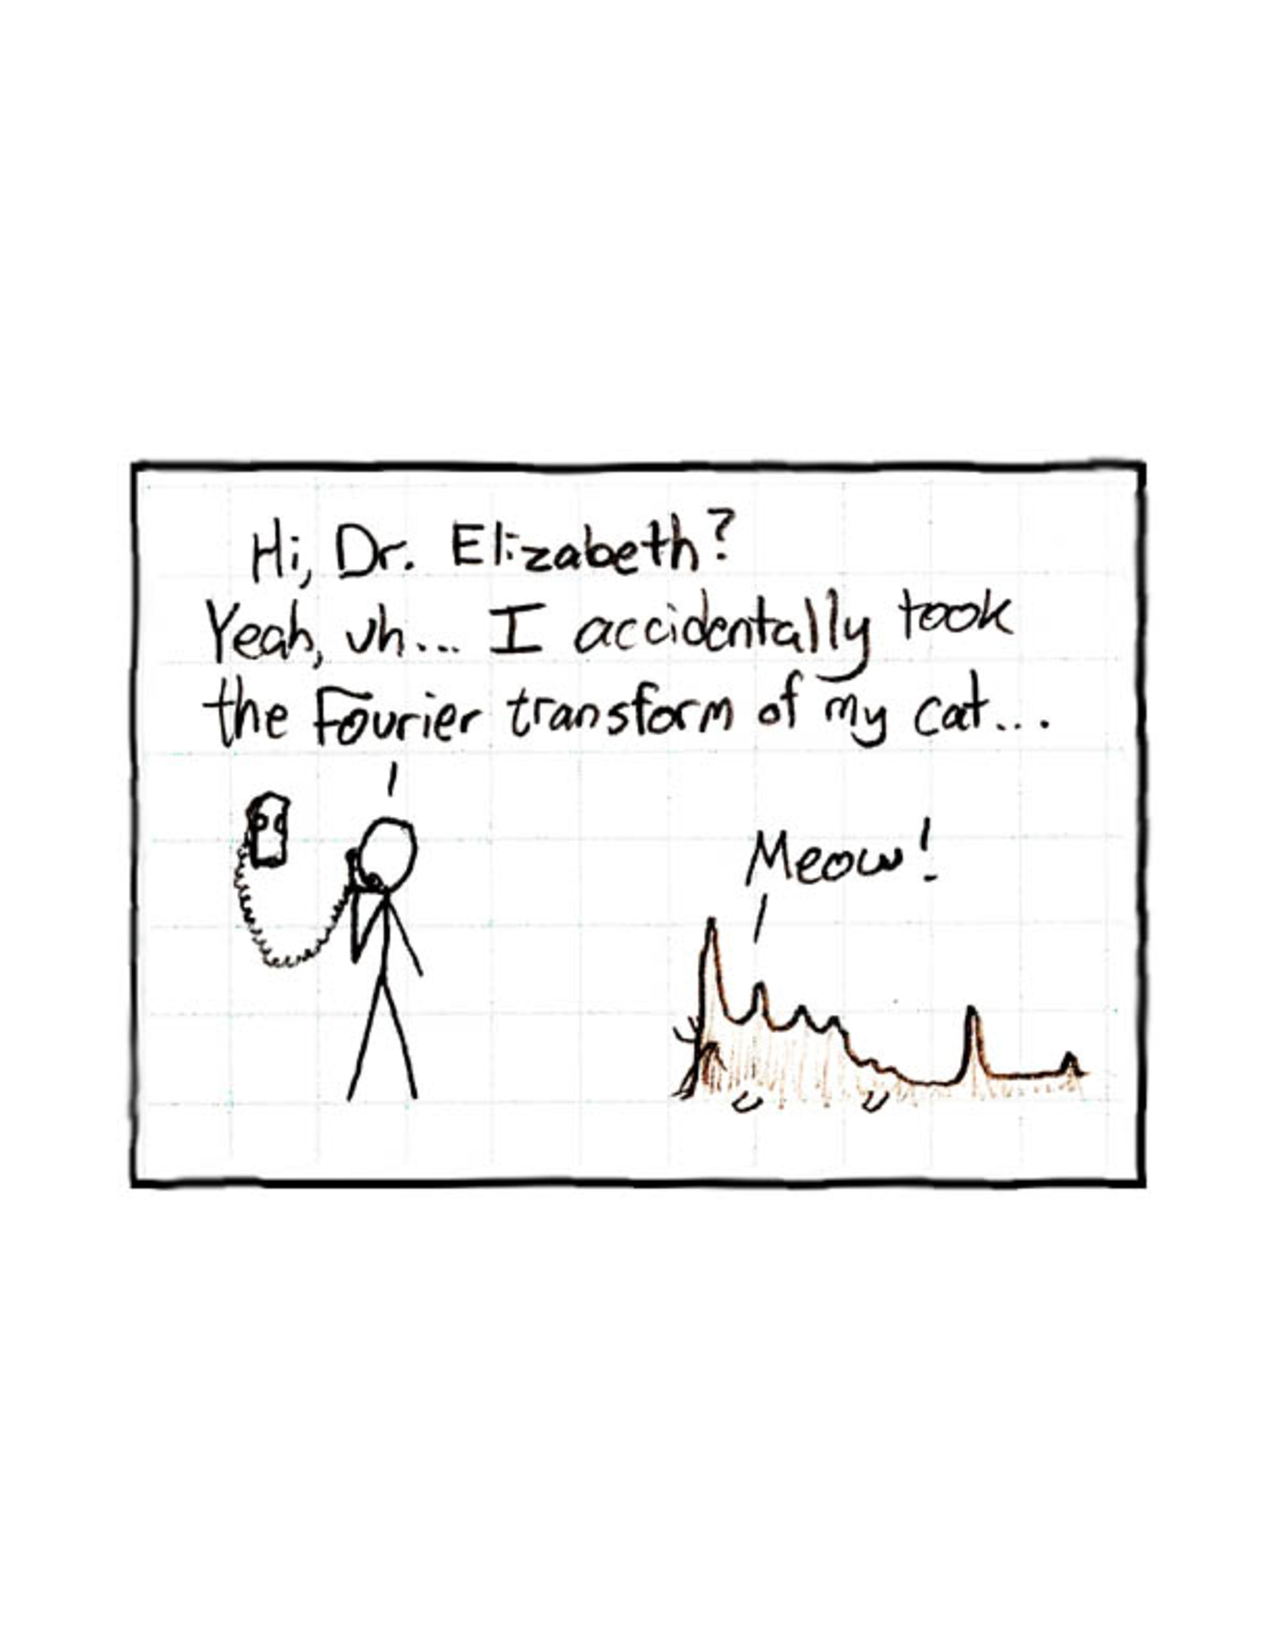
\includegraphics[width = 0.6\textwidth]{89-PS9-FourierComic}\\
	\copyright XKCD:  \url{https://imgs.xkcd.com/comics/fourier.jpg}
	\end{center}
	
	
\addfooter
%%%%%%%%%%%%%%%%%%%%%%%%%%%%%%%%%%%%%%%%%%%%%%%%%%%%%%%%%%%%%%%%%%%%%%%%%%%%%%%%
\end{document}


